% !TEX root = main.tex
The analysis is performed according to ISO14040, ISO14044 and ISO15804...

\begin{itemize}
	\item Impact category: GWP
	\item Functional unit: ${\mathrm{m^2}}$ (shading) and ${\mathrm{kWh}}$ (PV)
	\item Scope and system boundaries: embodied, operational, disposal
	\item Cut-off method used
	\item Recipe midpoint H allocation method
\end{itemize}




\begin{equation}
G=\frac{{\mathrm{GWP}}}{{\mathrm{I \cdot \eta  \cdot PR \cdot LT \cdot A}}}
\label{eq:solar}
\end{equation}



\begin{figure}[H]
\begin{center}
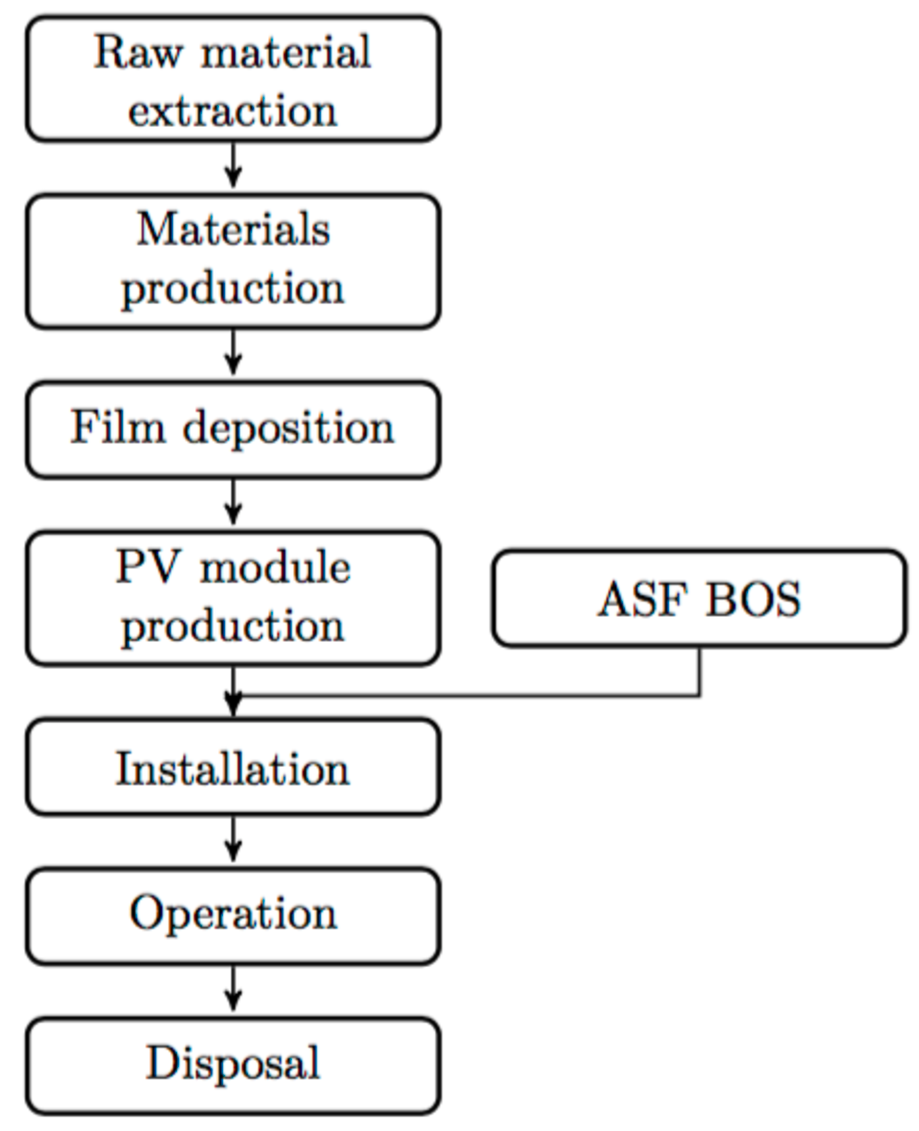
\includegraphics[width=5cm, trim= 0cm 0cm 0cm 0cm,clip]{BOS}
\caption{Thin-film incl. BOS (e.g. supporting structures and systems) analysis}
\label{fig:BOS}
\end{center}
\end{figure}



\begin{figure}[H]
\begin{center}
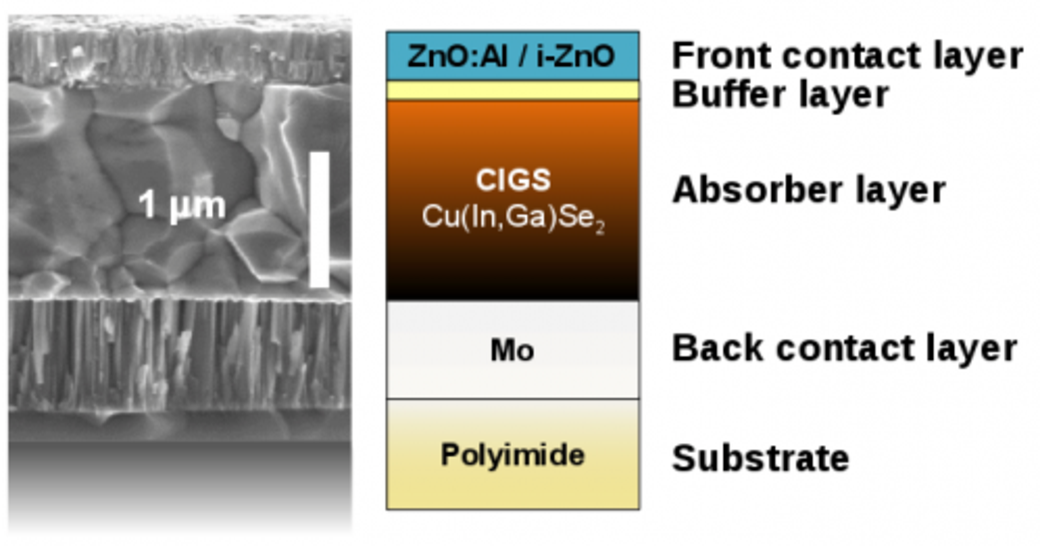
\includegraphics[width=8cm, trim= 0cm 0cm 0cm 0cm,clip]{schema}
\caption{CIGS thin film structure MAKE OWN GRAPH, DO NOT USE THIS ONE FOR FINAL}
\label{fig:schema}
\end{center}
\end{figure}

% \begin{enumerate}
% \item Solar irradiation Zurich, Switzerland: 1240 ${\mathrm{kWh/m^2/yr}}$
% \item Module efficiency CIGS: 11.5\%
% \item Performance ratio with optimal algorithm: 0.326\footnote{Based on full facade area of 8.96${\mathrm{m^2}}$; Actual PV film area only comprises of 5.76${\mathrm{m^2}}$}
% \item Electricity production: 46.54 ${\mathrm{kWh/m^2}}$; 417 ${\mathrm{kWh}}$
% \item Shading office room savings according to Table \ref{simulation} and \ref{netenergy}
% \item Lifetime: 15 years
% \item Maintenance every 5 years: 69.9 ${\mathrm{kg_{CO_2eq}}}$\footnote{Includes: baking and vacuuming actuator, actuator silicone, actuator mold and idling hoist for 8 hours}
% \item Disposal processes according to Appendix \ref{}
% \item Database source: Ecoinvent 3.1
% \end{enumerate}